\documentclass{beamer}
\usetheme{Boadilla}
\usepackage[utf8]{inputenc}
\usepackage{booktabs}
\usepackage{threeparttablex}
\usepackage{mathpazo}
\usepackage[mathpazo]{flexisym}
\usepackage{array}
\usepackage{caption}
\captionsetup[figure]{font=scriptsize}
\usepackage{graphicx}
\usepackage{threeparttablex}
\usepackage[labelformat=empty]{subfig}
\usepackage[T1]{fontenc}
\usepackage{tikz}

\newcommand\hd[2]{\multicolumn{2}{c}{\begin{tabular}{@{}c@{}}#2\end{tabular}}}
\newcolumntype{C}[1]{>{\centering\let\newline\\\arraybackslash\hspace{0pt}}m{#1}}
\let\estinput=\input
\newcommand{\estwide}[3]{
        \vspace{.75ex}{
            \textsymbols
            \begin{tabular*}
            {\textwidth}{@{\hskip\tabcolsep\extracolsep\fill}l*{#2}{#3}}
            \toprule
            \estinput{#1}
            \bottomrule
            \addlinespace[.75ex]
            \end{tabular*}
            }
        }

\newcommand{\estauto}[3]{
        \vspace{.75ex}{
            \textsymbols
            \begin{tabular}{l*{#2}{#3}}
            \toprule
            \estinput{#1}
            \bottomrule
            \addlinespace[.75ex]
            \end{tabular}
            }
        }

\newcommand{\specialcell}[2][c]{%
    \begin{tabular}[#1]{@{}c@{}}#2\end{tabular}
}

\definecolor{MyBackground}{rgb}{0.95,0.95,0.96}
\setbeamercolor{background canvas}{bg=MyBackground}

\definecolor{UniBlue}{RGB}{83,121,170}
\setbeamercolor{title}{fg=UniBlue}
\setbeamercolor{frametitle}{fg=UniBlue}
\setbeamercolor{structure}{fg=UniBlue}
\setbeamertemplate{footline}{}

\AtBeginSection[]{
  \begin{frame}
  \vfill
  \centering
  \begin{beamercolorbox}[sep=8pt,center,shadow=true,rounded=true]{title}
    \usebeamerfont{title}\insertsectionhead\par%
  \end{beamercolorbox}
  \vfill
  \end{frame}
}

\title[]{Project Workflow}
\date{}

\begin{document}

\maketitle

\beamertemplatenavigationsymbolsempty
\begin{frame}{Publishing in Economics - Process}
    \begin{itemize}
        \item Kitt Carpenter - \color{blue} \href{https://www.appam.org/how-many-journals-work-a-far-from-incomplete-guide-for-public-policyeconomics-scholars/?pg=58&F_All=y}{How (many) journals work}
    \end{itemize}
    \smallskip
    \begin{itemize}
        \item \textbf{Step 1: Pre-review check} 
        \begin{itemize}
            \item Primarily formatting
        \end{itemize}
        \item \textbf{Step 2: Managing editor review}
        \begin{itemize}
            \item ``Broad skim of paper for fit and quality'' (does not read entire paper)
            \item Does the paper merit peer review?
            \item Desk rejection phase
            \item Timing: 2 weeks to 2 months
        \end{itemize}
        \item \textbf{Step 3: Co-editor check}
        \begin{itemize}
            \item Managing editor assigns paper to a co-editor (\color{blue} \href{https://www.aeaweb.org/journals/aer/about-aer/editors}{example}\color{black})
            \item Co-editor is an expert in the paper's field (usually reads entire paper)
            \item Identifies reviewers and sends paper out for review
            \item Can still desk reject
            \item Timing: 2 to 6 months
        \end{itemize}
        \item \textbf{Step 4: Final decision}
        \begin{itemize}
            \item Co-editor evaluates reviewer comments (and their own thoughts on the paper) 
            \item Makes an accept/revise/reject decision or recommendation to the managing editor
        \end{itemize}
    \end{itemize}          
\end{frame}

\begin{frame}{Publishing in Economics - Sample Rates}
    \begin{figure}
        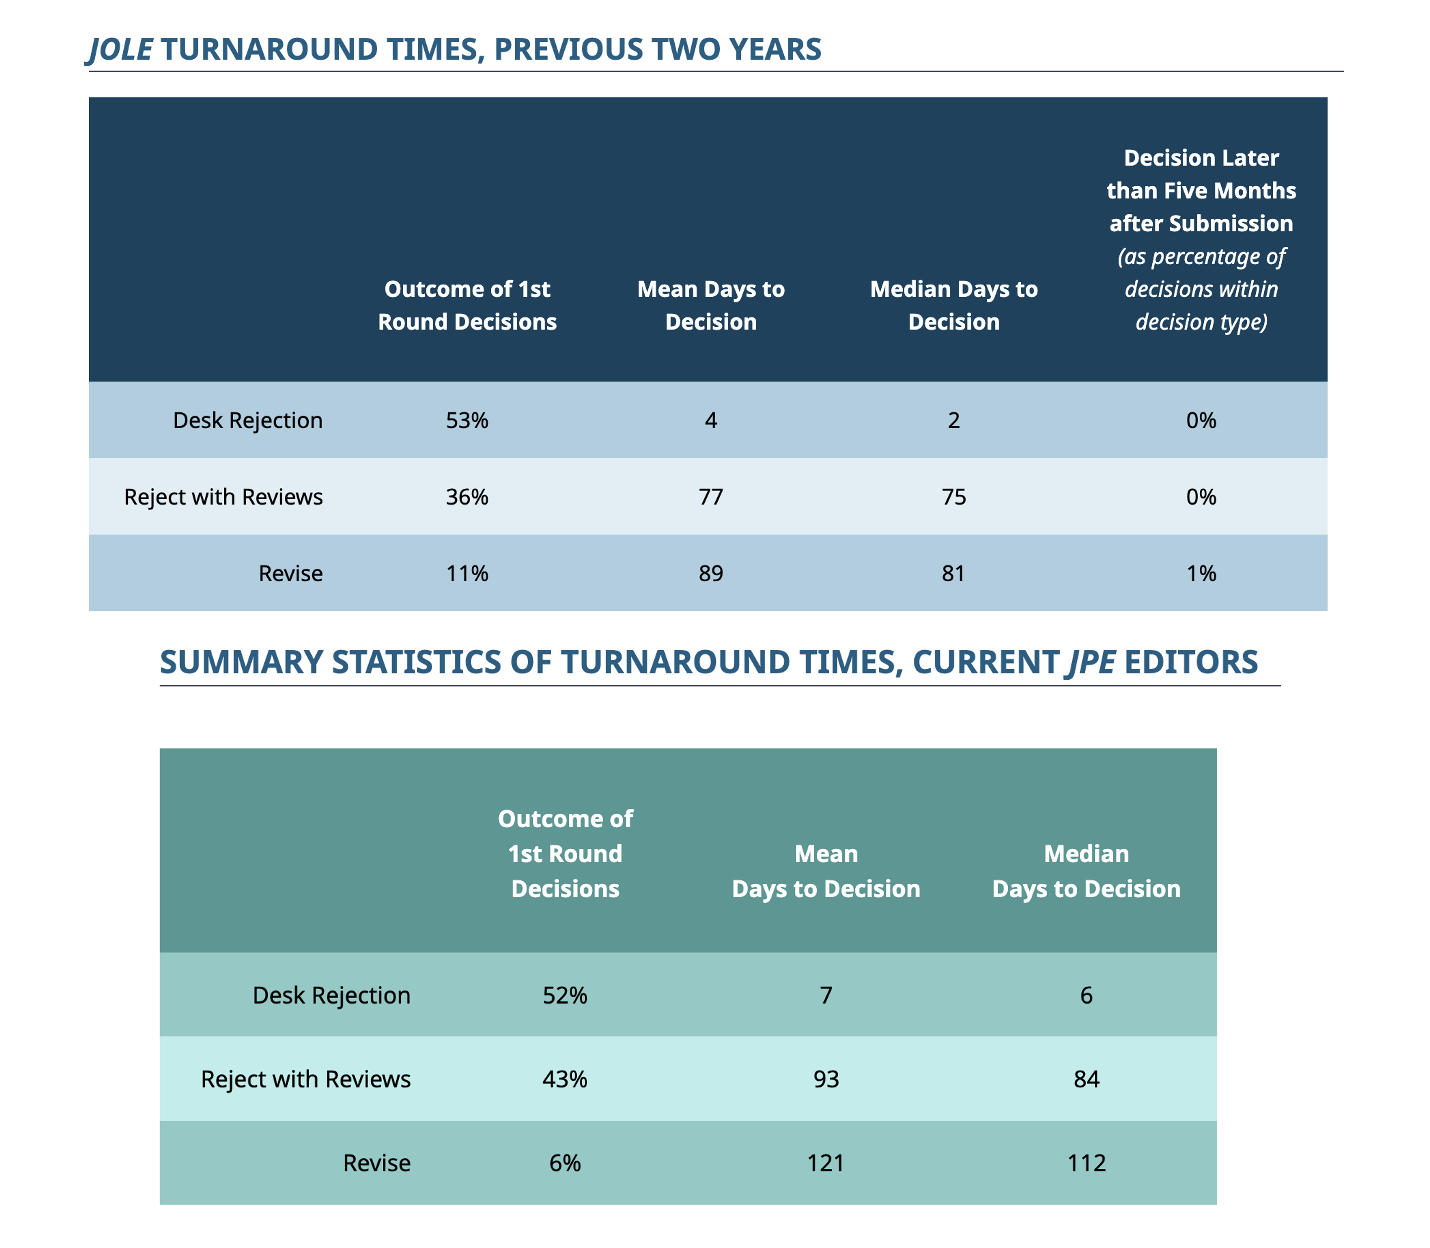
\includegraphics[scale=0.35]{/images/rates.png}
    \end{figure}      
\end{frame}

\end{document}